\documentclass{exam}
%%% BEGIN PREAMBLE

\usepackage{amsfonts}
\usepackage{amsthm}
\usepackage{hyperref}
\usepackage{graphicx}
\usepackage[german, english]{babel}
\usepackage[utf8]{inputenc}
\usepackage{amsmath}

\pointpoints{\%}{\%}
\newtheorem{theorem}{Theorem}
\theoremstyle{definition}
\newtheorem{example}{Example}


% Definitions
\theoremstyle{definition}
\newtheorem{remark}[theorem]{Remark}

\newcommand{\emptystring}{\varepsilon}
\newcommand{\length}[1]{\mid #1 \mid}
\newcommand{\directlygenerates}{\Rightarrow}
\newcommand{\generates}{\Rightarrow^{+}}
\newcommand{\generatesequal}{\Rightarrow^{*}}

\newenvironment{grammar}
	{\begin{tabular}[b]{lcl}}
	{\end{tabular}}
\newcommand{\rewritten}{$\to$}
\newcommand{\alternative}{$\mid$}

%\printanswers
%%% BEGIN DOCUMENT
\begin{document}

\begin{center} \fbox{\fbox{\parbox{5.5in}{\centering
Formal Languages Basic Terminology --- Exercises}}}
\end{center}
%\makebox[\textwidth]{Name: \enspace\hrulefill}

\begin{questions}

\question {\bf EBNF $\to$ Classical Grammar Notation}
	
	Given the following rule of a grammar of a programming language (in EBNF):
	
	\begin{otherlanguage}{german}
		Die folgende Grammatik einer Programmiersprache ist in EBNF gegeben:
	\end{otherlanguage}
	
	\begin{grammar}
		Stat & = & ``BEGIN" \{Stat\} ``END" \\
		& \alternative & ``IF" Expr ``THEN" Stat \\
		&& \{``ELSIF" Expr ``THEN" Stat\} \\
		&& [``ELSE" Stat] \\
		& \alternative & ``FOR" "var" ``:=" Expr (``TO" \alternative ``DOWNTO") Expr \\
		&& ``DO" Stat.
	\end{grammar}
	
	Transform this rule into the classical notation of formal languages as presented in class. Try to use
	understandable names for the non-terminals needed.

	\begin{otherlanguage}{german}
		Übertragen Sie diese Grammatik in die klassische Grammatiknotation. Nehmen Sie verständliche Namen
		für die Nonterminalsymbole.
	\end{otherlanguage}
	
\begin{solution}
	
		\begin{tabular}[b]{lcl}
			Stat & $\to$ & BEGIN StatSeq END \\
			StatSeq & $\to$ & Statement $\mid$ Statement StatSeq $\mid \varepsilon$ \\
			Statement & $\to$ & IfStatement $\mid$ ForStatement \\
			IfStatement & $\to$ & IF Expr THEN Stat ElseBlock \\
			ElseBlock & $\to$ & ElseIfBlock FinalElse \\
			ElseIfBlock & $\to$ & ELSEIF Expr THEN Stat ElseIfBlock $\mid \varepsilon$ \\
			FinalElse & $\to$ & ELSE Stat $\mid \varepsilon$ \\
			ForStatement & $\to$ & FOR var := Expr Direction Expr DO Stat \\
			Direction &$\to$ & TO $\mid$ DOWNTO
		\end{tabular}
	\end{solution}
	
\question {\bf Syntax Diagram $\to$ EBNF -- Constant}
Given the following rule of grammar of a constant in C in form of a syntax diagram.
	
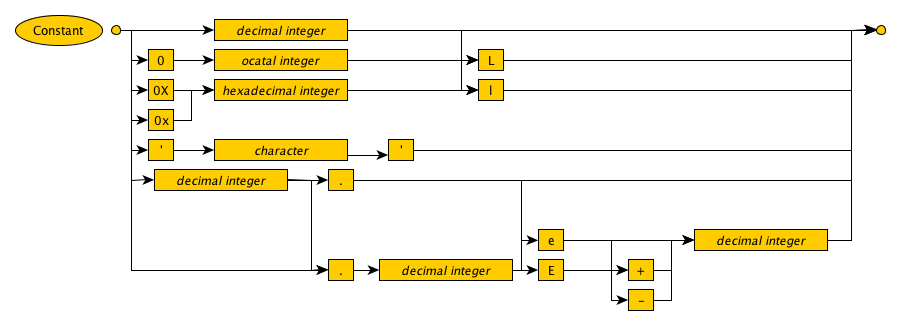
\includegraphics[scale=.5]{SyntaxDiagramConstant.png}
	
Rewrite this rule in EBNF according to the rules given in class.

\begin{otherlanguage}{german}
Geben Sie die in Form eines Syntaxdiagramms angegebene Grammatik einer Konstanten in C als EBNF an.
\end{otherlanguage}

	
\question{\bf Java if Statement}
Give the grammar of the Java if statement in EBNF. Take care to consider all cases with if, else, else if. You may use the non-terminals ``Statement'' and ``Condition''.

\begin{otherlanguage}{german}
	Geben Sie die Grammatik für das If-Statement in JAVA in EBNF an. Beachten Sie alle Fälle mit if, else if und else. Sie dürfen die Non-Terminal-Symbole ``Statement'' und ``Condition'' verwenden.
\end{otherlanguage}

\question{\bf Railway Train}
A railway  train is composed of one or more locomotives, then zero or more  goods trucks, then followed either by a guard's van or by one or more passenger coaches which then is followed by a guard's van (Begleitwagen). Describe this sequence in form of Wirth's EBNF. Use the following vocabulary $\Sigma =$ \{Locomotive, GoodsTruck, PassengerCoach, GuardsVan\}. If you need more symbols, just introduce them.

\begin{otherlanguage}{german}
Ein Eisenbahnzug besteht aus einer Reihe verschiedener Wagons. Er beginnt mit mindestens einer oder auch mehreren Lokomotiven, welche dann von null oder mehreren Güterwagons gefolgt werden. Nach diesen kann optional ein Begleitwagen kommen oder sofort eine Reihe von einem oder mehreren Personenwagons. Sind Personenwagons vorhanden, werden diese jedenfalls von einem Begleitwagen abgeschlossen.

Beschreiben Sie diese Folge in Form einer Wirth'schen EBNF. Sie können folgendes Alphabet benutzen: $\Sigma =$ \{Locomotive, GoodsTruck, PassengerCoach, GuardsVan\}. GuardsVan bedeutet Begleitwagen. Sie können $\Sigma$ aber auch erweitern, falls dies notwendig sein sollte.
\end{otherlanguage}

\begin{solution}

	\begin{grammar}
		RailwayTrain = Locomotive \{Locomotive\} \{GoodsTruck\} TrainRest. \\
		TrainRest = [PassengerCoach \{PassengerCoach\}]GuardsVan.
	\end{grammar}
\end{solution}
\end{questions}
\end{document}